\documentclass[11pt]{article}
\usepackage{acl2016}
\usepackage{times}
% \usepackage[round]{natbib}
\usepackage{latexsym}
\usepackage[utf8]{inputenc}
\usepackage[font=small,labelfont=bf]{caption}
\usepackage{amsmath}
\usepackage{multirow}
\usepackage{appendix}
\usepackage{url}
\usepackage{tikz}
% \usepackage{avm}
% \avmfont{\sc}
% \avmoptions{sorted}
% \avmvalfont{\rm}
% \avmsortfont{\scriptsize\it}
\usepackage{remreset}
\usepackage{pifont}
% \newcommand{\cmark}{\ding{53}}%
\usepackage{graphicx}
\usepackage{wrapfig}
\usepackage{verbatim} 
\usepackage{linguex}
\usepackage{qtree}
%\usepackage{algorithm}% http://ctan.org/pkg/algorithms
%\usepackage{algpseudocode}% http://ctan.org/pkg/algorithmicx
\usepackage{amsmath,amsfonts,amssymb}

\newcommand{\argmax}{\operatornamewithlimits{argmax}}

\usepackage{color}
\newcommand{\das}[1]{{\color{red}\emph{//das: #1//}}}
\newcommand{\crk}[1]{\emph{//crk: #1//}}
\newcommand{\todo}[1]{\textcolor{green}{\emph{//todo: #1//}}}


\newcommand{\sds}[0]{\textsc{sds}}
\newcommand{\nlu}[0]{\textsc{nlu}}
\newcommand{\rmrs}[0]{\textsc{rmrs}}
\newcommand{\ep}[0]{\texttt{EP}}
\newcommand{\inprotk}[0]{\textsc{InproTK}}
\newcommand{\sium}[0]{\textsc{sium}}
\newcommand{\asr}[0]{\textsc{asr}}
\newcommand{\dm}[0]{\textsc{dm}}
\newcommand{\ui}[0]{\textsc{gui}}
\newcommand{\iu}[0]{\textsc{iu}}
\newcommand{\rr}[0]{\textsc{rr}}
\newcommand{\conf}[0]{\textsc{conf}}
\newcommand{\pa}[0]{\textsc{pa}}


%Document Head
% \dochead{CLV2 Class File Manual}

%\title{An Adaptive, Incremental Personal Assistant that Graphically Signals Speech Understanding}
\title{Supporting Spoken Assistant Systems with a Graphical User\\ Interface that Signals Incremental Understanding and Prediction State}


\aclfinalcopy
\author{Casey Kennington \and David Schlangen\\Boise State University and DSG / CITEC / Bielefeld University}
% \affil{CITEC, Bielefeld University}


\begin{document}
% \affil{Publishing / SPi}

\maketitle

% abstract should be 150-250 words
\begin{abstract}
Arguably, spoken dialogue systems are most often used not in hands/eyes-busy situations, but rather in settings where a graphical display is also available, such as a mobile phone. We explore the use of a graphical output modality for signaling incremental understanding and prediction state of the dialogue system. By visualising the current dialogue state and possible continuations of it as a simple tree, and allowing interaction with that visualisation (e.g., for confirmations or corrections), the system provides both feedback on past user actions and guidance on possible future ones, and it can span the continuum from slot filling to full prediction of user intent (such as GoogleNow). We evaluate our system with real users and report that they found the system intuitive and easy to use, and that incremental and adaptive settings enable users to accomplish more tasks.
\end{abstract}

\section{Introduction}
\label{section:intro}

Current virtual personal assistants (\pa s) require users to either formulate complex intents in one utterance (e.g., ``call Peter Miller on his mobile phone'') or go through tedious sub-dialogues (e.g., ``phone call'' -- \emph{who would you like to call?} -- ``Peter Miller'' -- \emph{I have a mobile number and a work number. Which one do you want?}). This is not how one would interact with a human assistant, where the request would be naturally structured into smaller chunks that individually get acknowledged (e.g., ``Can you make a connection for me?'' -- \emph{sure} -- ``with Peter Miller'' - \emph{uh huh} - ``on his mobile'' - \emph{dialling now}). Current \pa s signal ongoing understanding by displaying the state of the recognised speech (\asr) to the user, but not their semantic interpretation of it. Another type of assistant system forgoes enquiring user intent altogether and infers \emph{likely} intents from context. GoogleNow, for example, might present traffic information to a user picking up their mobile phone at their typical commute time. These systems display their ``understanding'' state, but do not allow any type of interaction with it apart from dismissing the provided information.

In this work, we explore adding a graphical user interface (\ui) modality that makes it possible to see these interaction styles as extremes on a continuum, and to realise positions between these extremes and present a mixed graphical/voice enabled \pa\ that can provide feedback of understanding to the user \emph{incrementally} as the user's utterance unfolds--allowing users to make requests in instalments instead of fully thought-out requests. It does this by signalling ongoing understanding in an intuitive tree-like \ui\ that can be displayed on a mobile device. We evaluate our system by directing users to perform tasks using it under non-incremental (i.e., \asr\ endpointing) and incremental conditions and then compare the two conditions. We further compare a non-adaptive with an adaptive (i.e., infers likely events) version of our system. We report that the users found the interface intuitive and easy to use, and that users were able to perform tasks more efficiently with incremental as well as adaptive variants of the system.

\section{Related Work}
\label{section:related_work}

This work builds upon several threads of previous research: \newcite{Chai2014} addressed misalignments in understanding (i.e., common ground) \cite{clarkschaefer:contrdis} between robots and humans by informing the human of the internal system state via speech. We take this idea and apply it to a \pa\ by displaying the internal state of the system to the user via a \ui\ (explained in Section~\ref{section:display}), allowing the user to determine if system understanding has taken place--a way of providing feedback and backchannels to the user. \newcite{Dethlefs2015} provide a good review of work that show how backchannels facilitate grounding, feedback, and clarifications in human spoken dialogue, and apply an \emph{information density} approach to determining when to backchannel using speech. Because we don't backchannel using speech here, there is no potential overlap between the user and the system; rather, our system can display backchannels and ask clarifications without frustrating the user through inadvertent overlaps.

Though different in many ways, our work is similar in some regards to \newcite{Larsson2011}, which displays information to the user and allows the user to navigate the display itself (e.g., by saying \emph{up} or \emph{down} in a menu list)--functionality that we intend to apply to our \ui\ in future work. Our work is also comparable to \sds\ toolkits such as IrisTK \cite{Skantze2012a} and OpenDial \cite{Lison2015a} which enable \sds\ designers to visualize the internal state of their systems, though not for end user interpretability. 

Some of the work here is inspired by the \emph{Microsoft Language Understanding Intelligent Service} (LUIS) project \cite{Williams2015_sigdial}. While our system by no means achieves the scale that LUIS does, we offer here an additional contribution of an open source LUIS-like system (with the important addition of the graphical interface) that is authorable (using JSON files; we leave authoring using a web interface like that of LUIS to future work), extensible (affordances can be easily added), incremental (in that respect going beyond LUIS), trainable (i.e., can learn from examples, but can still function well without examples), and can learn through interacting (here we apply a user model that learns during interaction). 

\section{System Description}
\label{section:system_def}

This section introduces and describes our \sds, which is modularised into four main components: \asr, natural language understanding (\nlu), dialogue management (\dm), and the graphical user interface (\ui) which, as explained below, is visualised as a right-branching tree. The overall system is represented in Figure~\ref{fig:overview}. For the remainder of this section, each module is explained in turn. As each module processes input incrementally (i.e., word for word), we first explain our framework for incremental processing.

\begin{figure}[ht]
  \centering
      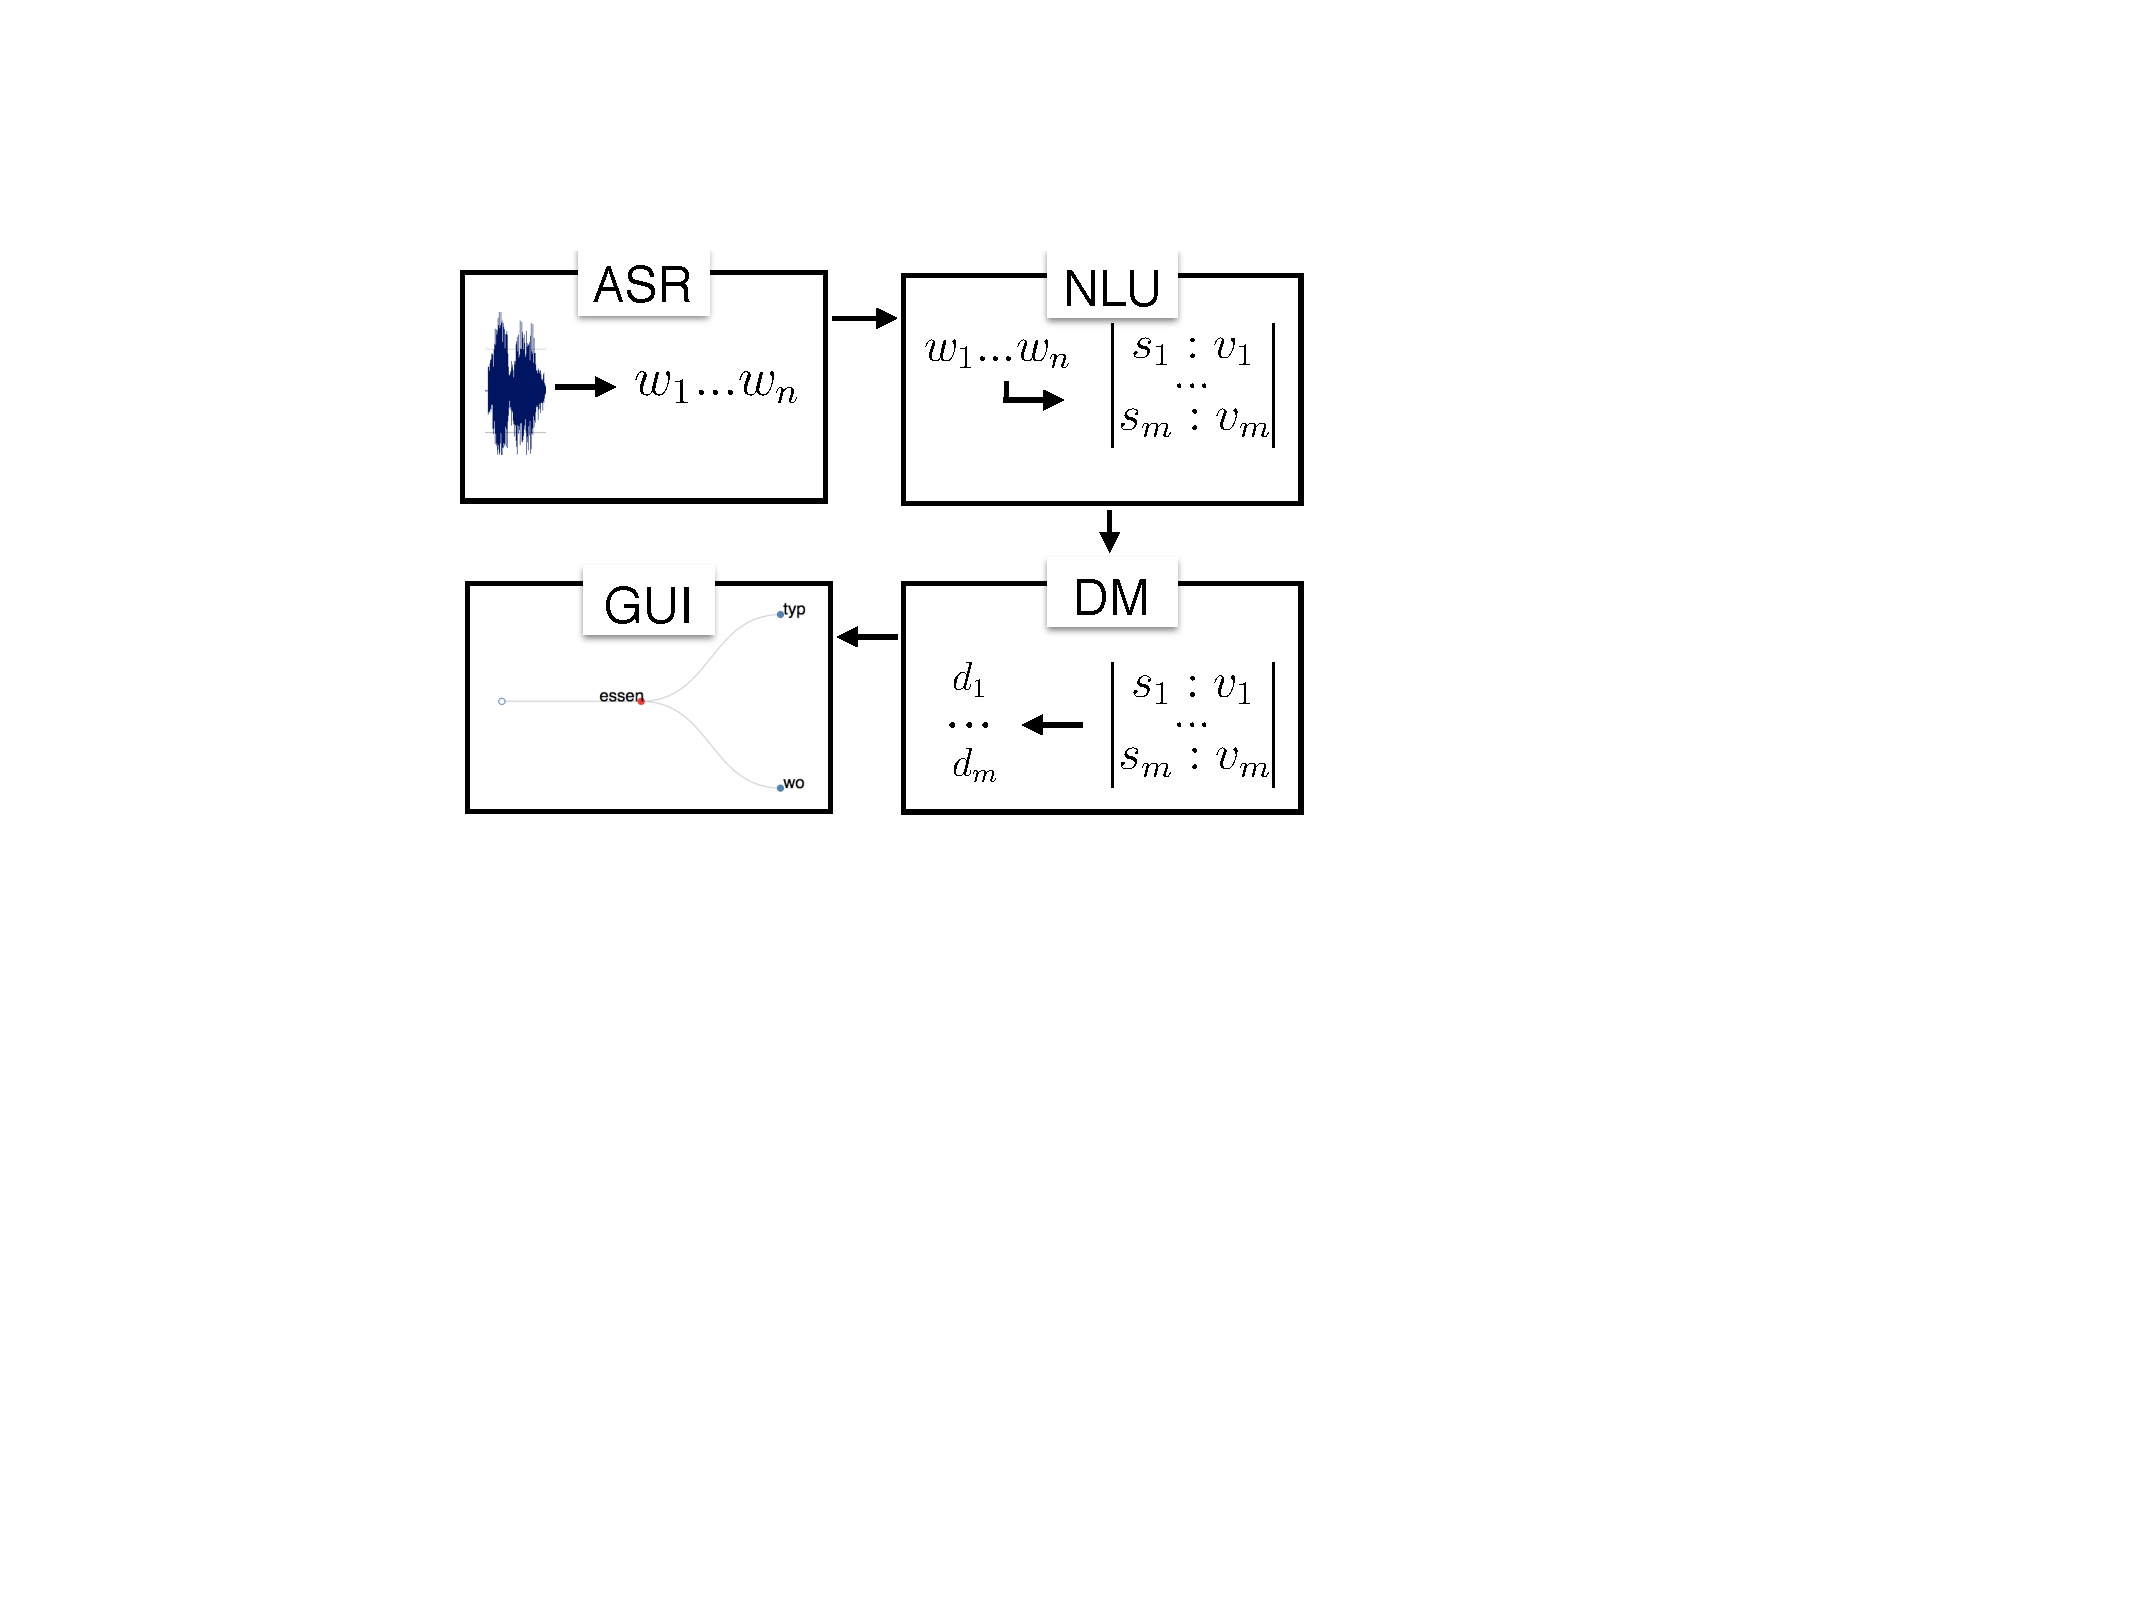
\includegraphics[width=0.5\textwidth]{figures/sig16-overview.pdf}	
      \caption{Overview of system made up of \asr\ which takes in a speech signal and produces transcribed words, \nlu, which takes words and produces a slots in a frame, \dm\ which takes slots and produces a decision for each, and the \ui\ which displays the state of the system. \label{fig:overview}}
\end{figure}


\subsection{Incremental Dialogue}

An aspect of our \sds\ that sets it apart from others is the requirement that it process \emph{incrementally}. One potential concern with incremental processing is regarding informativeness: why act early when waiting might provide additional information, resulting in better-informed decisions? The trade off is \emph{naturalness} as perceived by the user who is interacting with the \sds. Indeed, it has been shown that human users perceive incremental systems as being more natural than traditional, turn-based systems \cite{Aist2006,Skantze2009,skantze2010sigdial,Asri2014}, offer a more human-like experience  \cite{Edlund2008b} and are more satisfying to interact with than non-incremental systems \cite{Aistetal:incrunder-short}. Psycholinguistic research has also shown that humans process (i.e., comprehend) utterances as they unfold and do not wait until the end of an utterance to begin the comprehension process \cite{Tanenhaus1995,Spivey_2002tw}. 

The trade-off between informativeness and naturalness can be reconciled when mechanisms are in place that allow earlier decisions to be repaired. Such mechanisms are offered by the incremental unit (\iu) framework for \sds\ \cite{Schlangen2011}, which we apply here. Following \newcite{kennington-kousidis-schlangen:2014:W14-43}, the \iu\ framework consists of a network of processing \emph{modules}. A typical module takes input, performs some kind of processing on that data, and produces output. The data are packaged as the payload of \emph{incremental units} (\textsc{iu}s) which are passed between modules. The \textsc{iu}s themselves are interconnected via so-called \emph{same level links} (\textsc{sll}) and \emph{grounded-in links} (\textsc{grin}), the former allowing the linking of \textsc{iu}s as a growing sequence, the latter allowing that sequence to convey what \textsc{iu}s directly affect it (see Figure \ref{fig:iu_example} for an example of incremental \asr). Thus \iu s can be \emph{added}, but can be later \emph{revoked} and replaced in light of new information. The \iu\ framework can take advantage of up-to-date information, but have the potential to function in such a way that users perceive as more natural.

\begin{figure} %[ht]
  \centering
      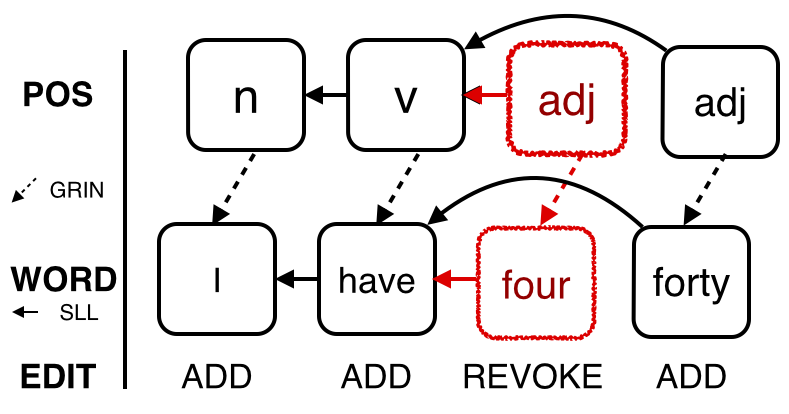
\includegraphics[width=0.45\textwidth]{figures/005_iu_example.png}	
      \caption{Example of IU network; part-of-speech tags are grounded into words, tags and words have same level links with left IU; \emph{four} is revoked and replaced with \emph{forty}.\label{fig:iu_example}}
            \vspace{-0.25cm}
\end{figure}

The modules explained in the remainder of this section are implemented as \iu-modules and process incrementally. Each will now be explained. 

\subsection{Speech Recognition}

The module that takes speech input from the user in our \sds\ is the \asr\ component. Incremental \asr\ must transcribe uttered speech into words which must be forthcoming from the \asr\ as early as possible (i.e., the \asr\ must not wait for endpointing to produce output). Each module that follows must also process incrementally, acting in lock-step upon input as it is received. Incremental \asr\ is not new \cite{baumannetal2009:naacl} and many of the current freely-accessible \asr\ systems can produce output (semi-) incrementally. We opt for Google \asr\ for its vocabulary coverage of our evaluation language (German). Following, \newcite{Baumann16}, we package output from the Google service into \iu s which are passed to the \nlu\ module, which we now explain. 

\subsection{Language Understanding}

We approach the task of \nlu\ as a slot-filling task (a very common approach; see \newcite{Tur2012}) where an intent is complete when all slots of a \emph{frame} are filled. The main driver of the \nlu\ in our \sds\ is the \sium\ model of \nlu\ introduced in \newcite{Kennington2013a}. \sium\ has been used in several systems which have reported substantial results in various domains, languages, and tasks \cite{Han2015,Kennington2015_naacl,Kennington2016} Though originally a model of reference resolution, it was always intended to be used for general \nlu, which we do here. The model is formalised as follows:

\vspace{-0.25cm}
{\small
\begin{center}
\begin{equation}
   P(I|U) = \frac{1}{P(U)} P(I)\sum_{r\in R} P(U|R=r)P(R=r|I) 
\label{eq:disc1}
\end{equation}
\end{center}
}

That is, $P(I|U)$ is the probability of the intent $I$ (i.e., a frame slot) behind the speaker's (ongoing) utterance $U$. This is recovered using the mediating variable $R$, a set of \emph{properties} which map between aspects of $U$ and aspects of $I$. We opt for abstract properties here (e.g., the frame for \texttt{restaurant} might be filled by a certain type of cuisine intent such as \texttt{italian} which has properties like \texttt{pasta}, \texttt{mediterranean}, \texttt{vegetarian}, etc.). Properties are pre-defined by a system designer and can match words that might be uttered to describe the intent in question. For $P(R|I)$, probability is distributed uniformly over all properties that a given intent is specified to have. (If other information is available, more informative priors could be used as well.) The mapping between properties and aspects of $U$ can be learned from data. During application, $R$ is marginalised over, resulting in a distribution over possible intents.\footnote{In \newcite{Kennington2013a} the authors apply Bayes' Rule to allow $P(U|R)$ to produce a distribution over properties, which we adopt here.} This occurs at each word increment, where the distribution from the previous increment is combined via $P(I)$, keeping track of the distribution over time. 

All properties in $R$ receive probaibility mass from the learned sub-model $P(U|R)$, but to allow our system to function with minimal amounts of training data, we apply a simple rule: if some $r \in R$ and $w \in U$ are such that $r\doteq w$  (where $\doteq$ is string equality; e.g., an intent has the property of \texttt{pasta} and the word \emph{pasta} is uttered), then $P(U$=$w|R$=r$)$=$1$. To allow for possible \asr\ errors, we also apply an edit distance calculation between the words from \asr\ and the properties using \emph{Levenshtein distance} ($ld$) on the character sequences: $P(U$=$w|R$=$r)$=$1 - ld(w,r) / max(len(w),len(r))$ where the $ld$ is normalised by the length of the longest sequence (but we only apply this if the calculated value is above a threshold of 0.6; i.e., the two strings are mostly similar). Applying these three steps produces a distribution for $P(U|R)$, which is re-normalised to sum to one.

We apply an instantiation of \sium\ for each slot. The candidate slots that are processed depends on the state of the \ui\ (described below); only slots represented by visible nodes are considered, thereby reducing the possible frames that could be predicted. At each word increment, the updated slots (and their corresponding) distributions are given to the \dm, which will now be explained. 

\subsection{Dialogue Manager}

The \dm\ plays a crucial role in our \sds: as well as determining \emph{how} to act, the \dm\ is called upon to decide \emph{when} to act, effectively giving the \dm\ the control over timing of actions rather than relying on \asr\ endpointing--further separating our \sds\ from other systems. The \dm\ policy is based on a confidence score derived from the \nlu\ (in this case, we used the distribution's argmax value) using thresholds for \texttt{wait}, \texttt{confirm} and \texttt{select} set by hand (i.e., trial and error). At each word and resulting distribution from \nlu, the \dm\ needs to choose one of the following:

\begin{itemize}
 \item \texttt{wait} -- wait for more information (i.e., for the next word) %don't act until more information is forthcoming
 \item \texttt{select} -- as the \nlu\ is confident enough, fill the slot can with the argmax from \nlu %the \nlu\ is confident enough that a slot can be filled with the argmax for this slot from \nlu.
 \item \texttt{request} -- signal a (yes/no) clarification request on the current slot and the proposed filler%the dialogue has reached a state where the system has asked for a (yes/no) clarification request
 \item \texttt{confirm} -- act on the confirmation of the user; in effect, \texttt{select} the confirmed slot value%the user has responded to the clarification request (which acts similar to a \texttt{select})
\end{itemize}

Though the thresholds are statically set, we applied OpenDial \cite{Lison2015a} as an \iu-module to perform the task of the \dm\ with the future goal that these values could be adjusted through reinforcement learning (which OpenDial could provide). The \dm\ processes and makes a decision for \emph{each slot}, with the assumption that only one slot out of all that are processed will result in an non-\texttt{wait} action (though this is not enforced). 



\subsection{Graphical User Interface}
\label{section:display}

The goal of the \ui\ is to intuitively inform the user about the internal state of the ongoing understanding. One motivation for this is that the user can determine if the system understood the user's intent before providing the user with a response (e.g., a list of restaurants of a certain type); i.e., if any misunderstanding takes place, it happens before the system commits to an action and is potentially more easily repaired. 

\begin{wrapfigure}{r}{0.2\textwidth}
  \centering
      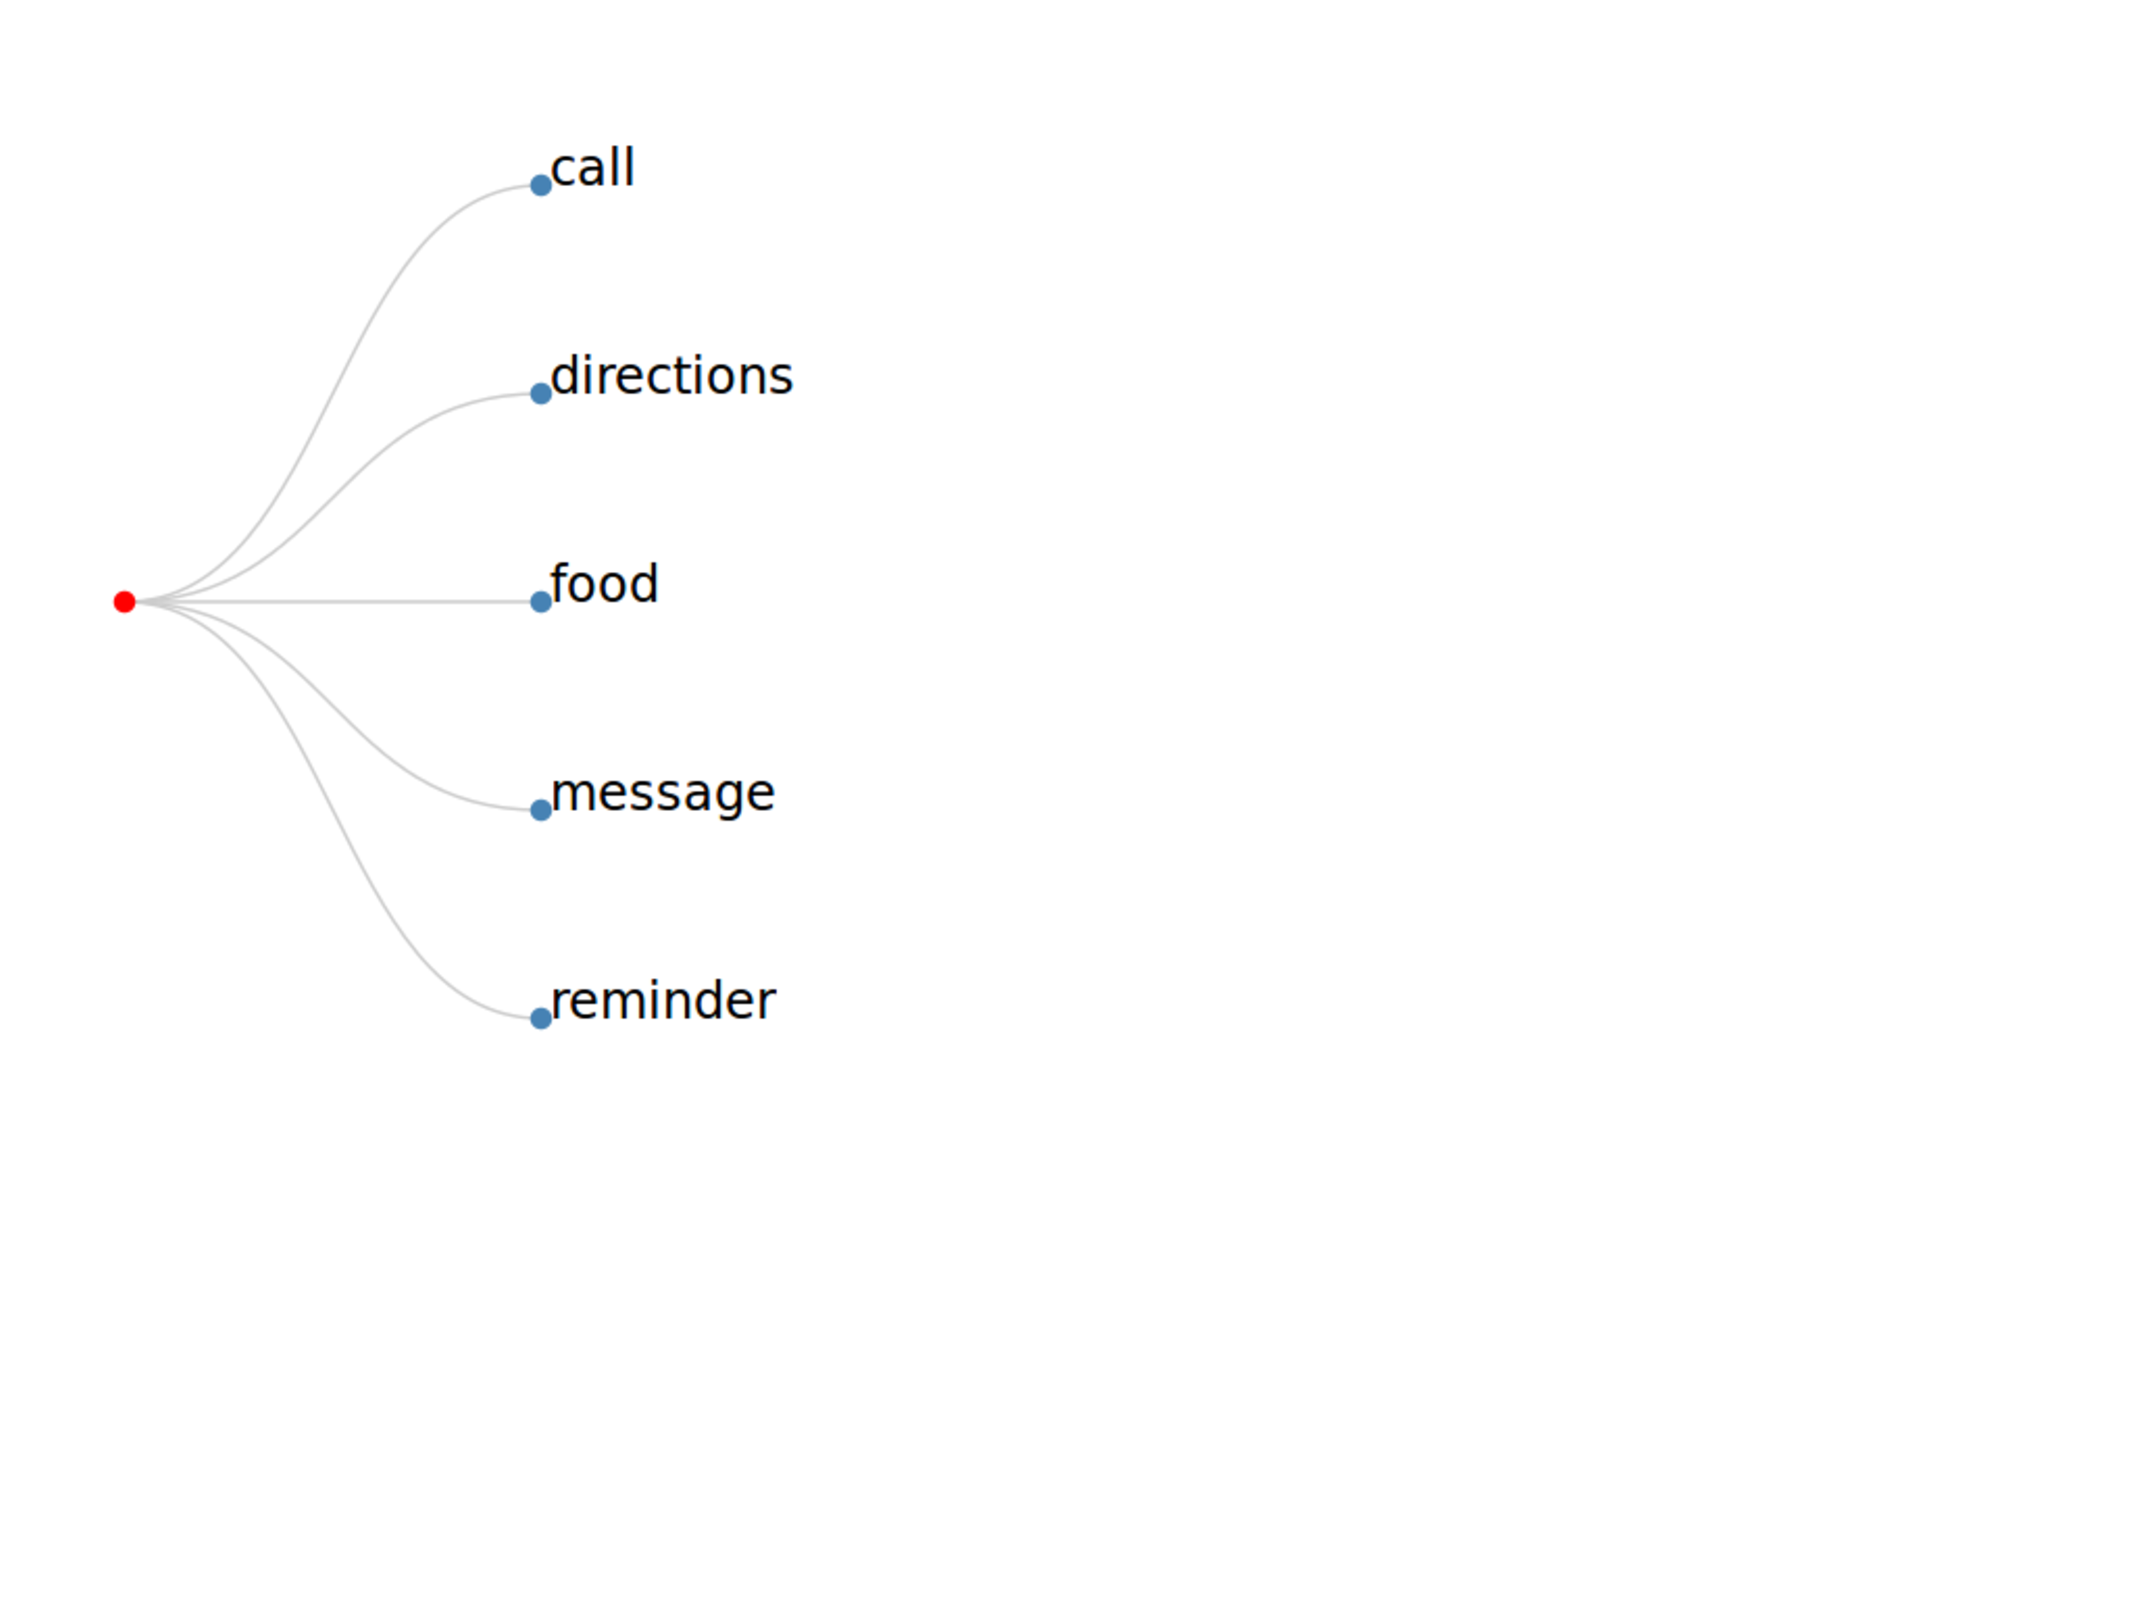
\includegraphics[width=0.2\textwidth]{figures/diatree-affordances.pdf}	
      \caption{Example tree as branching from the root; each branch represents a system affordance (i.e., making a phone call, reminder, finding a restaurant, leaving a message, and finding a route). \label{fig:affordances}}
\end{wrapfigure}

The display is a right-branching tree, where the branches directly off the root node display the affordances of the system (i.e., what domains of things it can understand and do something about). When the first tree is displayed, it represents a state of the \nlu\ where none of the slots are filled, an example of which is shown in Figure~\ref{fig:affordances}. 

When a user verbally selects a domain to ask about, the tree is adjusted to make that domain the only one displayed and the slots that are required for that domain are shown as branches. The user can then fill those slots (i.e., branches) by uttering the displayed name, or, alternatively, by uttering the item to fill the slot directly. For example, at a minimum, the user could utter the name of the domain then an item for each slot (e.g.,  \emph{food Thai downtown}) or the speech could be more natural (e.g., \emph{I'm quite hungry, I am looking for some Thai food maybe in the downtown area}). Crucially, the user can also hesitate within and between chunks, as advancement is not triggered by silence thresholding, but rather semantically.
When something is uttered that falls into the \texttt{request} state of the \dm\ as explained above, the display expands the subtree under question and marks the item with a question mark (see Figure~\ref{fig:confirm}). At this point, the user can utter any kind of confirmation. A positive confirmation fills the slot with the item in question. A negative confirmation retracts the question, but leaves the branch expanded. The expanded branches are displayed according to their rank as given by the \nlu's probability distribution. Though a branch in the display can theoretically display an unlimited number of children, we opted to only show 7 children; if a branch had more, the final child displayed as an ellipsis. 

\begin{figure}[ht]
  \centering
      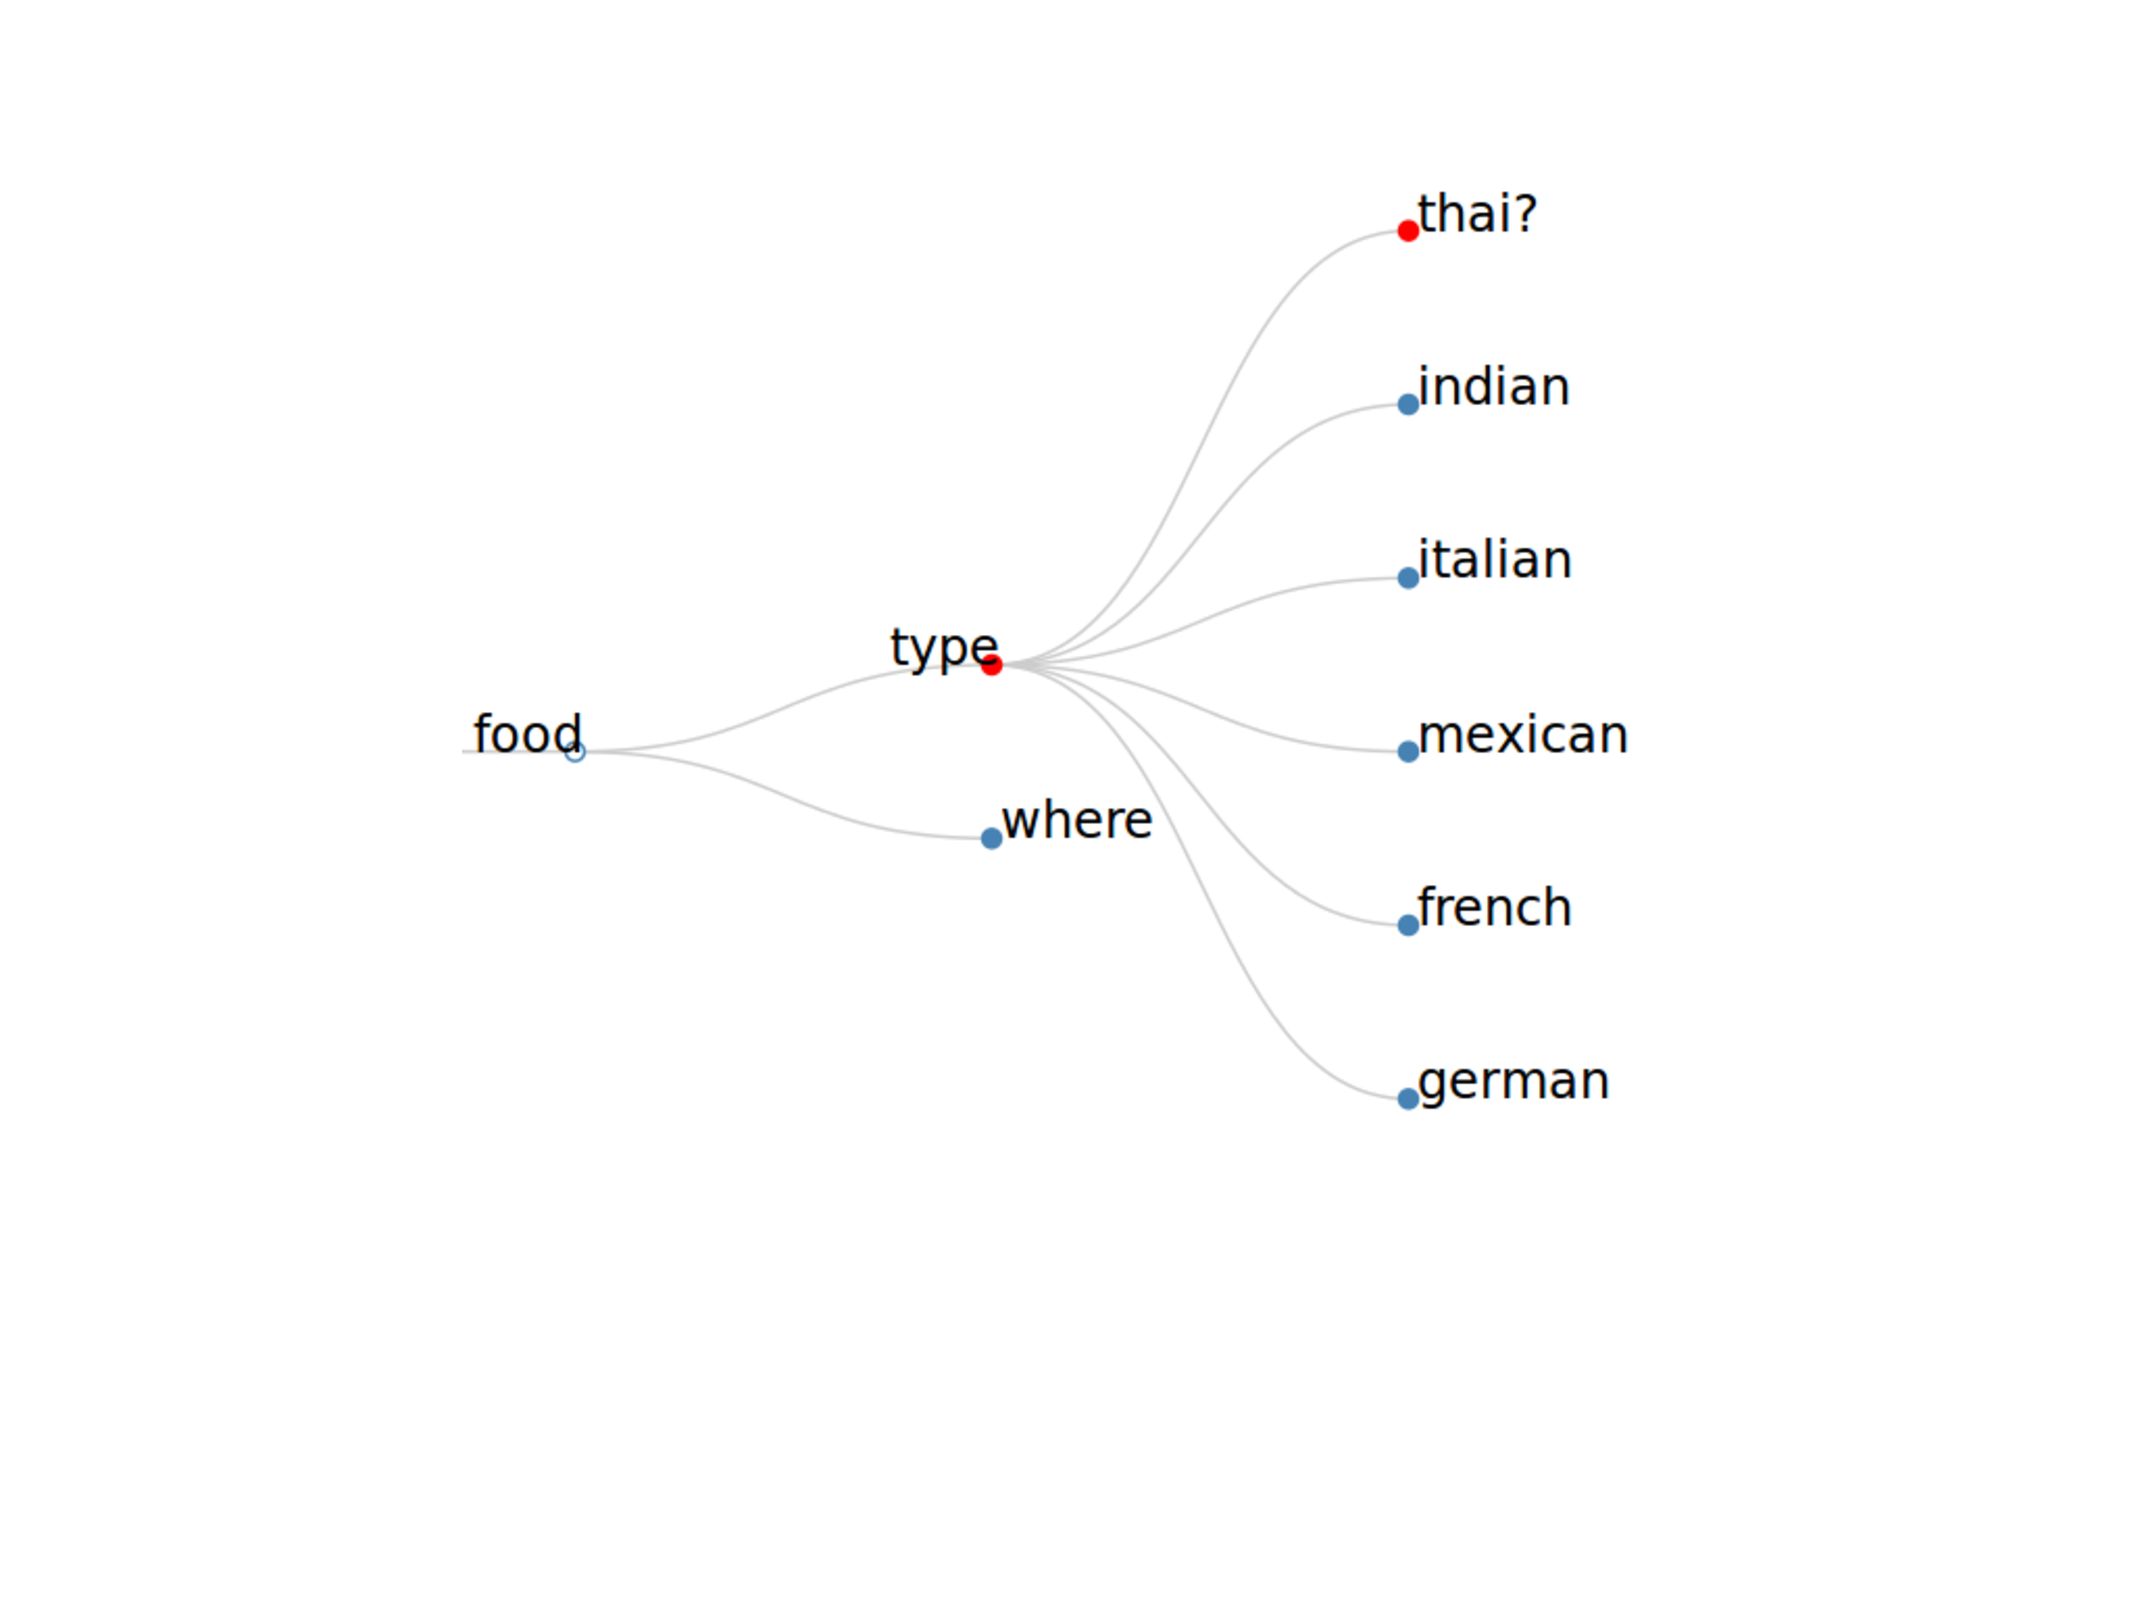
\includegraphics[width=0.5\textwidth]{figures/diatree-confirmation.pdf}	
      \caption{Example tree asking for confirmation on a specific node (in red with a question mark).\label{fig:confirm}}
\end{figure}

A completed branch is collapsed, visually marking its corresponding slot as filled. At any time, a user can backtrack by saying \emph{no} (or equivalent) or start the entire interaction over from the beginning with a keyword, e.g., \emph{restart}. To aid the user's attention, the node under question is marked in red, where completed slots are represented by outlined nodes, and filled nodes represent candidates for the current slot in question (see examples of all three in Figure~\ref{fig:confirm}). For cases where the system is in the \texttt{wait} state for several words (during which there is no change in the tree), the system signals activity at each word by causing the red node in question to temporarily change to white, then back to red (i.e., appearing as a blinking node to the user). Figure~\ref{fig:filled} shows a filled frame, represented as tree with one branch for each filled slot.

\begin{figure}[ht]
  \centering
      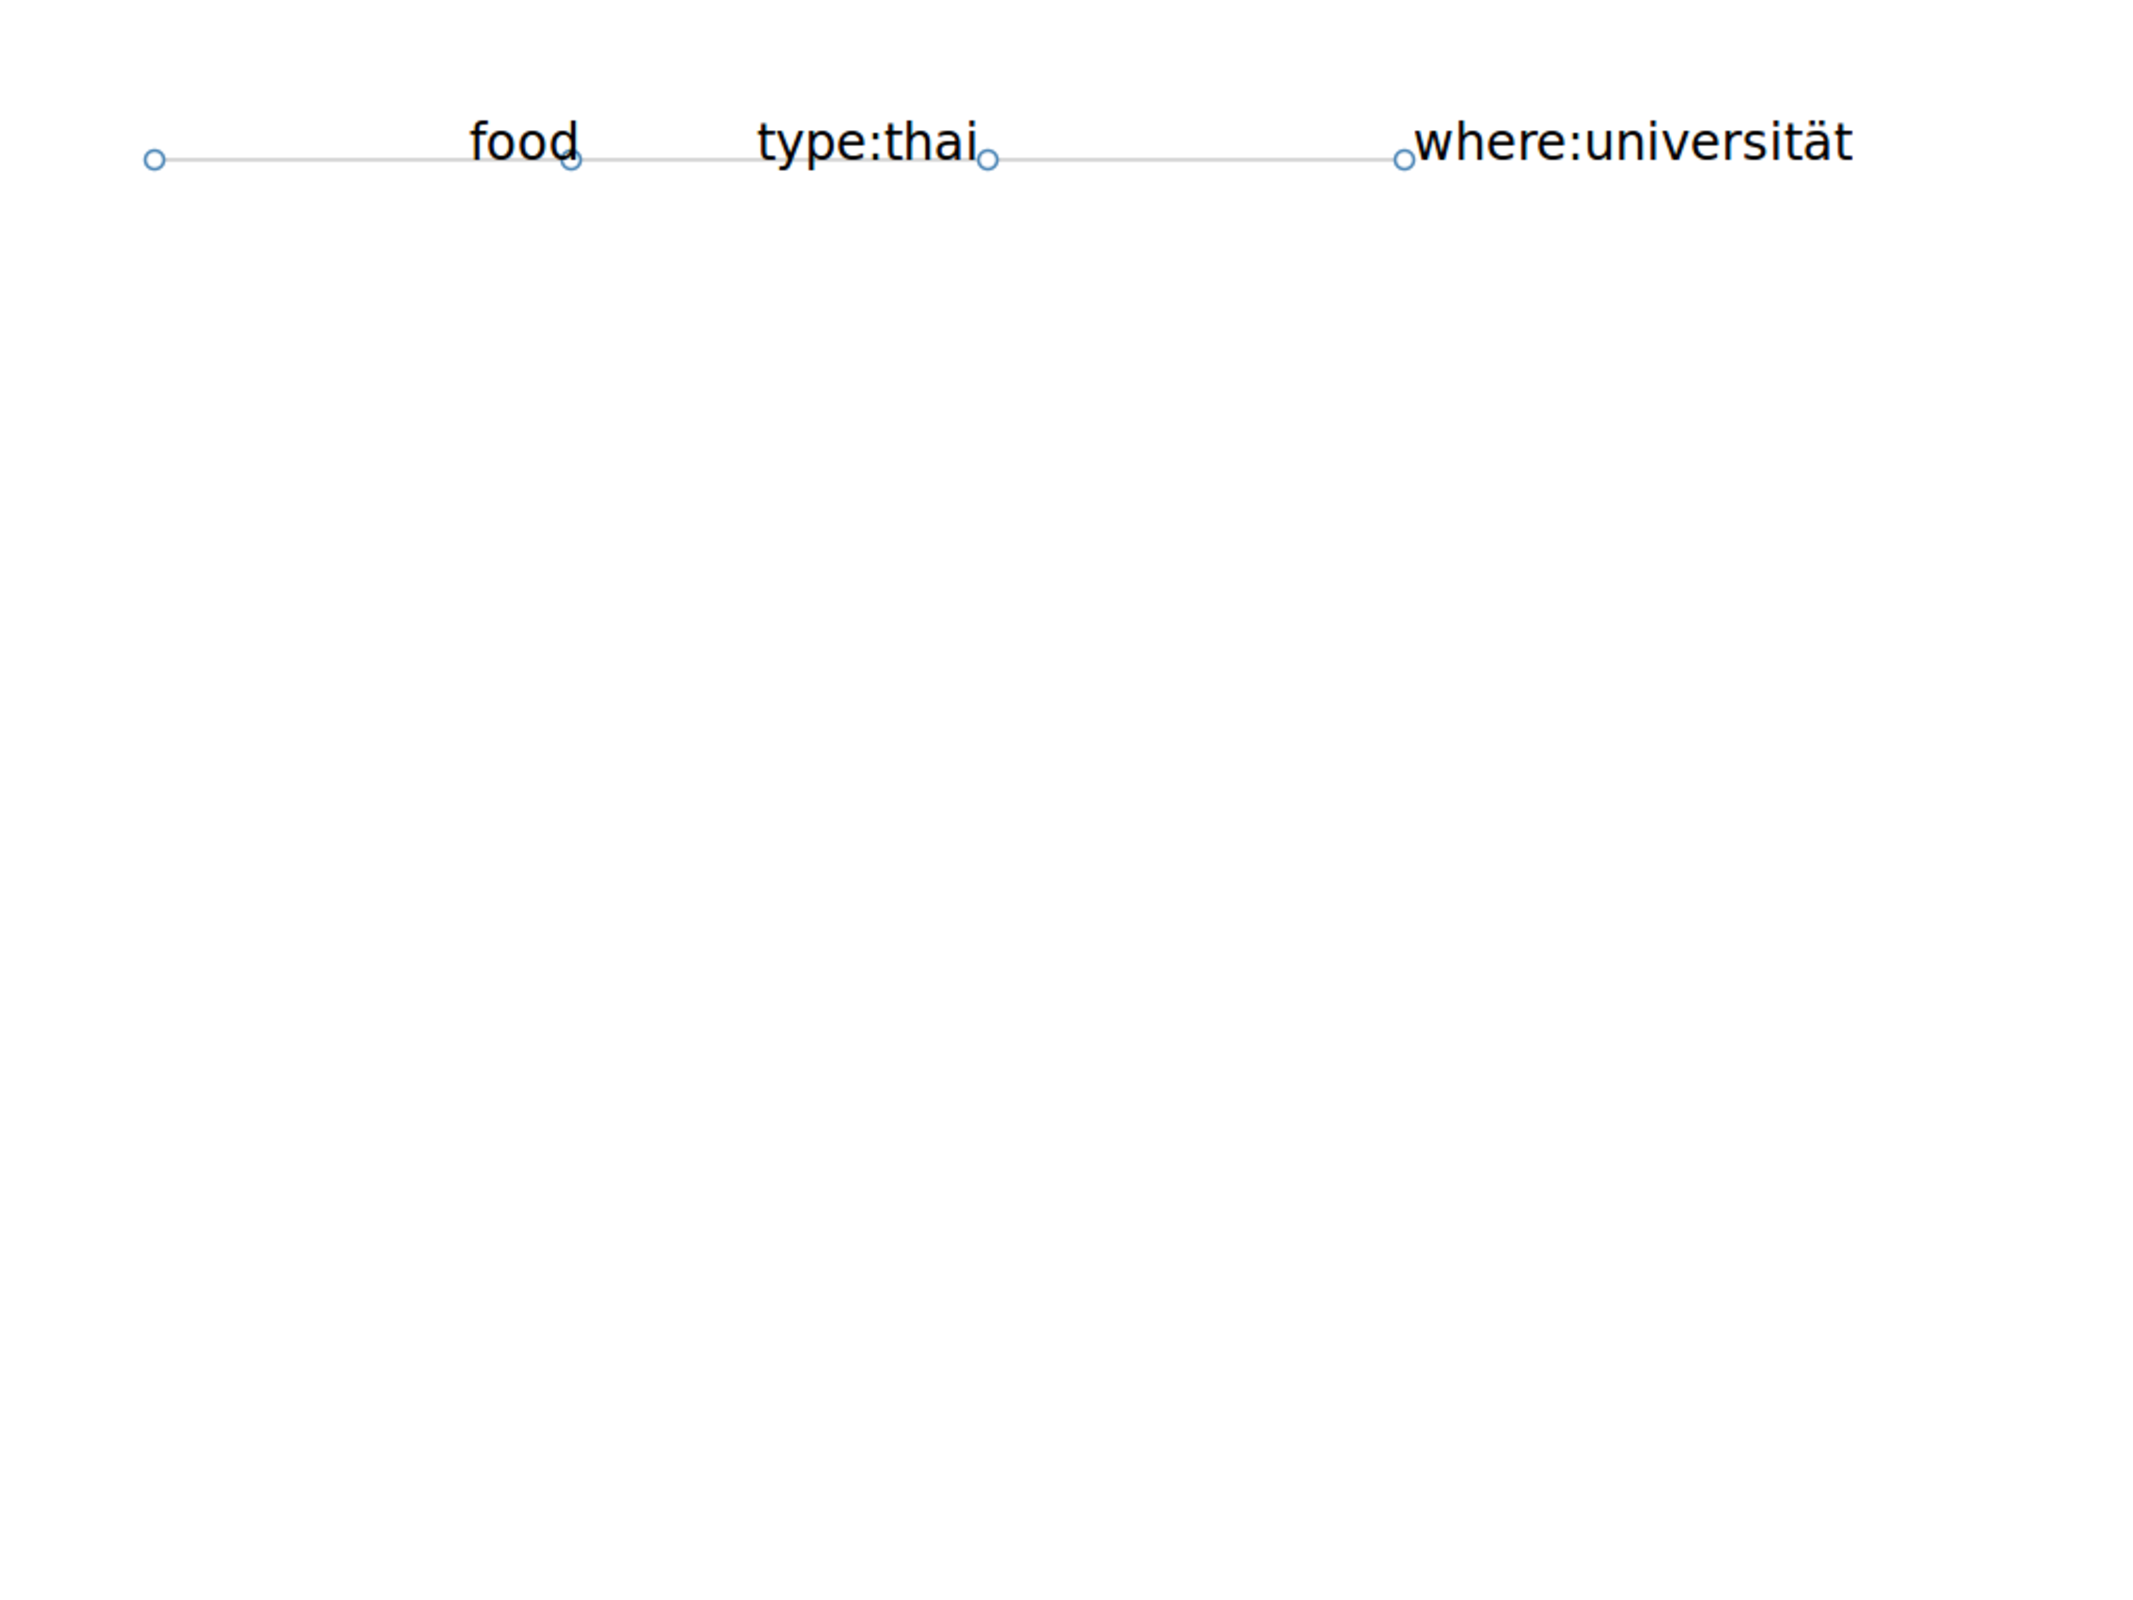
\includegraphics[width=0.45\textwidth]{figures/diatree-filled.pdf}	
      \caption{Example tree where all of the slots are filled. (i.e., \texttt{domain:food}, \texttt{location:university}, \texttt{type:thai}) \label{fig:filled}}
\end{figure}

Such an interface clearly shows the internal state of the \sds\ and whether or not it has understood the request so far. It is designed to aid the user's attention to the slot in question, and clearly indicates the affordances that the system has. The interface is currently a read-only display that is purely speech-driven, but it could be augmented with additional functionalities, such as tapping a node for expansion or typing input that the system might not yet display. It is currently implemented as a web-based interface (using the JavaScript D3 library), allowing it to be usable as a web application on any machine or mobile device. 

\paragraph{Adaptive Branching} The \ui\ as explained affords an additional straight-forward extension: the \ui\ can be used to signal what the system thinks the user might say next. This is done by expanding a branch and displaying a confirmation on that branch, signalling that the system predicts that the user will choose that particular branch. Alternatively, if the system is confident that a user will fill a slot with a particular value, that particular slot can be filled without confirmation. This is displayed as a collapsed tree branch. A system that perfectly predicts a user's intent would fill an entire tree (i.e., all slots) only requiring the user to confirm once. A more careful system would confirm at each step (such an interaction would only require the user to utter confirmations and nothing else). 


\section{Experiments}
\label{section:experiments}

In this section, we describe two experiments where we evaluated our system. It is our primary goal to show that our \ui\ is useful and signals understanding to the user. We also wish to show that incremental presentation of such a \ui\ is more effective than an endpointed system. We further want to show that an adaptive system is more effective than a non-adaptive system (though both would process incrementally). In order to best evaluate our system, we recruited participants to interact with our system in varied settings to compare endpointed (i.e., non-incremental) and non-adaptive as well as adaptive versions. We describe how the data were collected from the participants, then explain each experiment and give results.

\subsection{Task \& Procedure} 
\label{section:task_procedure}

\begin{wrapfigure}{r}{0.25\textwidth}
  \centering
      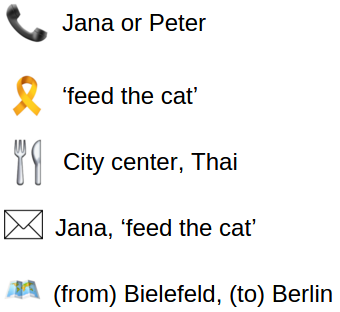
\includegraphics[width=0.25\textwidth]{figures/taskexample.png}	
      \caption{Examples of tasks, as presented to each participant. Each icon represents a specific task domain (i.e., call, reminder, find a restaurant, leave a message, or directions).\label{fig:taskex}}
\end{wrapfigure}

The participants were seated at a desk and given written instructions indicating that they were to use the system to perform as many tasks as possible in the allotted time. Figure~\ref{fig:taskex} shows some example tasks as they would be displayed (one at a time) to the user. A screen, tablet, and keyboard were on the desk in front of the user (see Figure~\ref{fig:dataview}).\footnote{We used a Samsung 8.4 Pro tablet turned to its side to show a larger width for the tree to grow to the right. The tablet only showed the \ui; the \sds\ ran on a separate computer.}  The user was instructed to convey the task presented on the screen to the system such that the \ui\ on the tablet would have a completed tree (e.g., as in Figure~\ref{fig:filled}). When the participant was satisfied that the system understood her intent, she was to press space bar on the keyboard which triggered a new task to be displayed on the screen and reset the tree to its start state on the tablet (as in Figure~\ref{fig:affordances}). 

The possible task domains were \emph{call}, which had a single slot for \emph{name} to be filled (i.e., one out of the 22 most common German given names); \emph{message} which had a slot for \emph{name} and a slot for the \emph{message} (which, when invoked, would simply fill in directly from the \asr\ until 1 second of silence was detected); \emph{eat} which had slots for \emph{type} (in this case, 6 possible types) and \emph{location} (in this case, 6 locations based around the city of Bielefeld); \emph{route} which had slots for \emph{source} city and the \emph{destination} city (which shared the same list of the top 100 most populous German cities); and \emph{reminder} which had a slot for \emph{message}. 

%Some of the slot types were shared across domains, such as \emph{message} (across \emph{reminder} and \emph{message}), \emph{name} (across \emph{message} and \emph{call}), as well as \emph{source} and \emph{destination} which shared the same list of German city names (the top 100 most populous cities). 

For each task, the domain was first randomly chosen from the 5 possible domains, and then each slot value to be filled was randomly chosen (the \emph{message} slot for the \emph{name} and \emph{message} domains was randomly selected from a list of 6 possible ``messages'', each with 2-3 words; e.g., \emph{feed the cat}, \emph{visit grandma}, etc.). The system kept track of which tasks were already presented to the participant. At any time after the first task, the system could choose a task that was previously presented and present it again to the participant (with a 50\% chance) so the user would often see tasks that she had seen before (with the assumption that humans who use \pa s often do perform similar, if not the same, tasks more than once). 

\begin{figure}[ht]
  \centering
      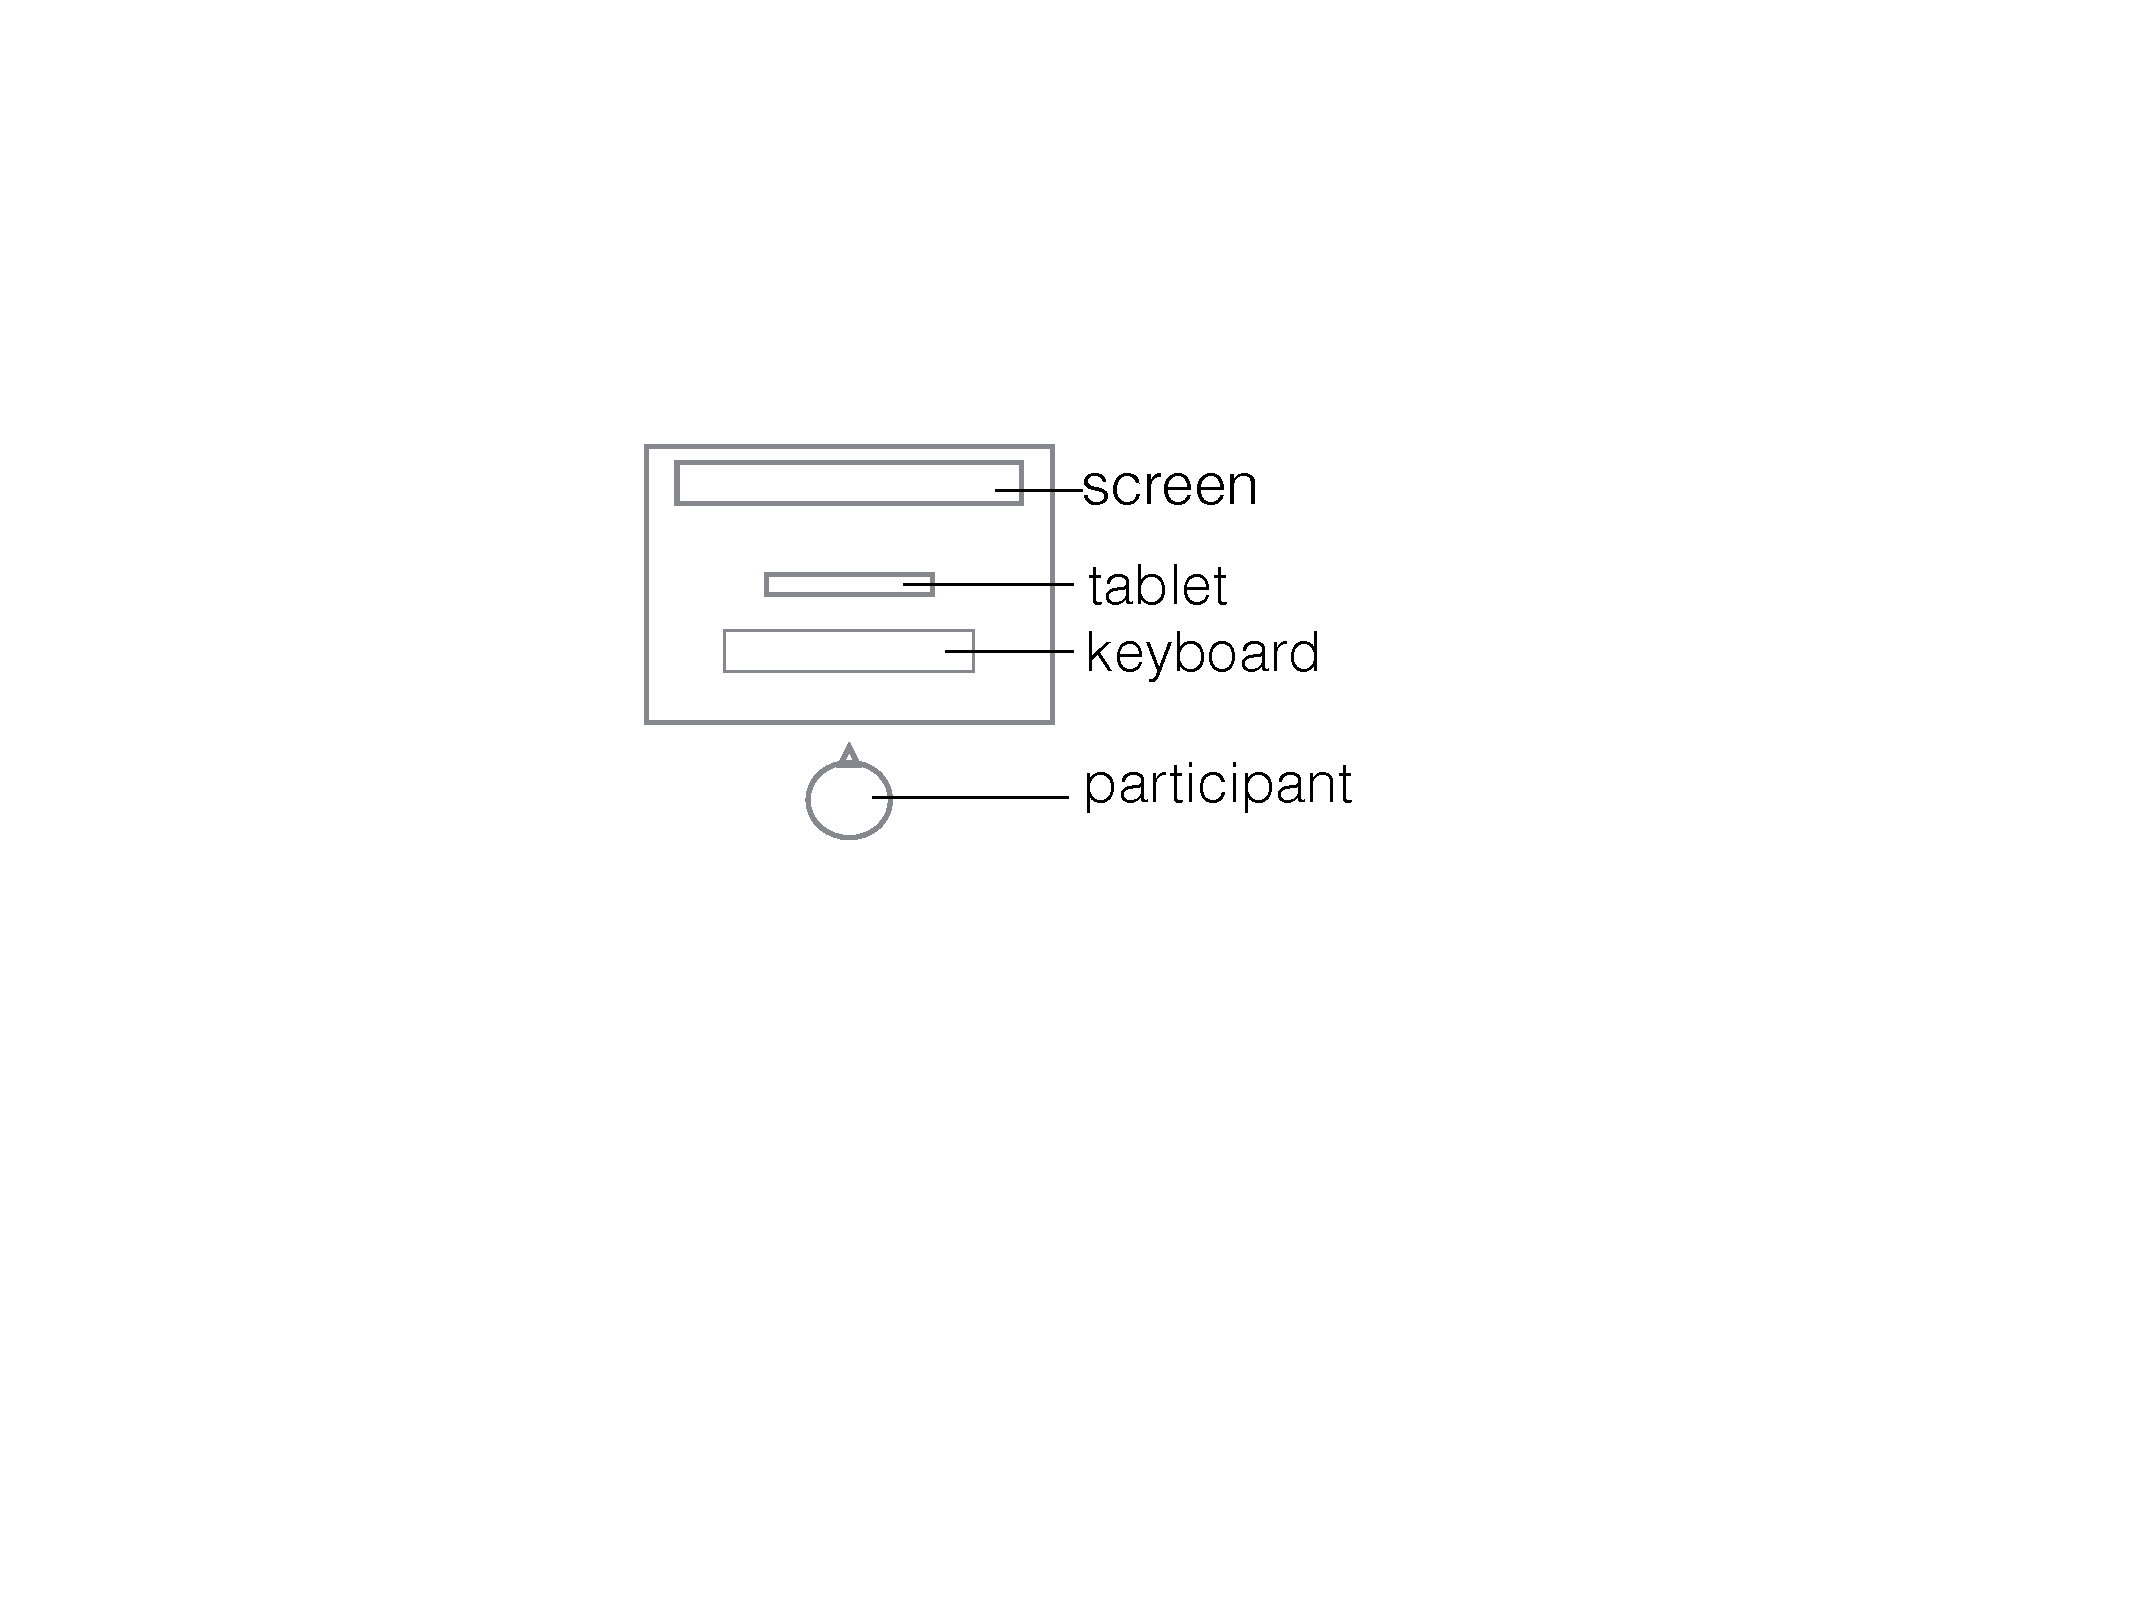
\includegraphics[width=0.4\textwidth]{figures/dataview.pdf}	
      \caption{Bird's eye view of the experiment: the participant sat at a table with a screen, tablet, and keyboard in front of them. \label{fig:dataview}}
\end{figure}

The participant was told that she would interact with the system in three different phases, each for 4 minutes, and to accomplish as many tasks as possible in that time allotment. The participant was not told what the different phases were. The experiments described in Sections~\ref{section:exp1} and \ref{section:exp2} respectively describe and report a comparison first between the Phase 1 and 2 (denoted as the \emph{endpointed} and \emph{incremental} variants of the system) in order to establish whether or not the incremental variant produced better results than the endpointed variant. We also report a comparison between Phase 2 and 3 (\emph{incremental} and \emph{incremental-adaptive} phases). Each of these phases are described below. Before the participant began Phase 1, they were able to try it out for up to 4 minutes (in Phase 1 settings) and ask questions about how it worked, allowing them to get used to the interface before the actual experiment began. After this trial phase, the experiment began with Phase 1. The phases were presented in the same order to all participants. We opted to not randomise the order or the presentation of the phases 

\paragraph{Phase 1: Non-incremental} In this phase, the system did not appear to work incrementally; i.e., the system displayed tree updates after \asr\ endpointing (of 1.2 seconds--a reasonable amount of time to expect a response from a commercial spoken \pa). The system displayed the ongoing \asr\ on the tablet as it was recognised (as is often done in commercial \pa s). At the end of Phase 1, a pop up window notified the user that the phase was complete. They then moved onto Phase 2.

\paragraph{Phase 2: Incremental} In this phase, the system displayed the tree information incrementally without endpointing. The \asr\ was no longer displayed; only the tree provided feedback in understanding, as explained in Section~\ref{section:display}. 

After Phase 2, a 10-question questionnaire was displayed on the screen for the participant to fill out comparing Phase 1 and Phase 2. For each question, they had the choice of \emph{Phase 1}, \emph{Phase 2}, \emph{Both}, and \emph{Neither}. (See Appendix for full list of questions.) After completing the questionnaire, they moved onto Phase 3.

\paragraph{Phase 3: Incremental-adaptive} In this phase, the incremental system was again presented to the participant with an added user model that ``learned'' about the user. If the user saw a task more than once, the user model would predict that, if the user chose that task domain again (e.g., \emph{route}) then the system would automatically ask a clarification using the previously filled values (except for the \emph{message} slot, which the user always had to fill). If the user saw a task more than 3 times, the system skipped asking for clarifications and filled in the domain slots completely, requiring the user only to press the space bar to confirm it was the correct one (i.e., to complete the task). An example progression might be as follows: a participant is presented with the task \emph{route from Bielefeld to Berlin}, then the user would attempt to get the system to fill in the tree (i.e., slots) with those values. After some interaction in other domains, the user sees the same task again, and now after indicating the intent type \emph{route}, the user must only say ``yes'' for each slot to confirm the system's prediction. Later, if the task is presented a third time, when entering that domain (i.e, \emph{route}), the two slots would already be filled. If later a different route task was presented, e.g., \emph{route from Bielefeld to Hamburg}, the system would already have the two slots filled, but the user could backtrack by saying ``no, to Hamburg'' which would trigger the system to fill the appropriate slot with the corrected value. Later interactions within the \emph{route} domain would ask for a clarification on the \emph{destination} slot since it has had several possible values given by the participant, but continue to fill the \emph{from} slot with \emph{Bielefeld}.

After Phase 3, the participants were presented with another questionnaire on the screen to fill out with the same questions (plus two additional questions), this time comparing Phase 2 and Phase 3. For each item, they had the choice of \emph{Phase 2}, \emph{Phase 3}, \emph{Both}, and \emph{Neither}. At the end of the three phases and questionnaires, the participants were given a final questionnaire to fill out by hand on their general impressions of the systems. 

We recruited 14 participants for the evaluation. We used the Mint tools data collection framework \cite{kousidis2012evaluating} to log the interactions. Due to some technical issues, one of the participants did not log interactions. We collected data from 13 participants, post-Phase 2 questionnaires from 12 participants,  post-Phase 3 questionnaires from all 14 participants, and general questionnaires from all 14 participants. In the experiments that follow, we report objective and subjective measures to determine the settings that produced superior results.

\paragraph{Metrics} We report the subjective results of the participant questionnaires. We only report those items that were statistically significant (see Appendix for a full list of the questions). We further report objective measures for each system variant: total number of completed tasks, fully correct frames, average frame f-score, and average time elapsed (averages are taken over all participants for each variant; we only used the 10 participants who fully interacted with all three phases). Discussion of the two experiments is left to the end of this section.

\subsection{Experiment 1: Endpointed vs. Incremental}
\label{section:exp1}

In this section we report the results of the evaluation between the \emph{endpointed} (i.e., non-incremental; Phase 1) variant vs the incremental (Phase 2) variant of our system.

\paragraph{Subjective Results} We applied a multinomial test of significance to the results, treating all four possible answers as equally likely (with Bonferroni correction of 10). The item \emph{The interface was useful and easy to understand} with the answer of \emph{Both} was significant ($ \chi^2 $ (4, N = 12) = 9.0, p $<$ .005), as was \emph{The assistant was easy and intuitive to use} also with the answer \emph{Both} ($ \chi^2 $ (4, N = 12) = 9.0, p $<$ .005). The item \emph{I always understood what the system wanted from me} was also answered \emph{Both} significantly more times than other answers ($ \chi^2 $ (4, N = 14) = 9.0, p $<$ .005), similarly for \emph{It was sometimes unclear to me if the assistant understood me} with the answer of \emph{Both} ($ \chi^2 $ (4, N = 12) = 10.0, p $<$ .005).  These responses tell us that though the participants did not report preference for either system variant, they reported a general positive impression of the \ui\ (in both variants). This is a nice result; the \ui\ could be used in either system with benefit to the users.

\paragraph{Objective Results}  The \emph{endpointed} (Phase 1) and \emph{incremental} (Phase 2) columns in Table~\ref{tab:objscores} show the results of the objective evaluation. Though the average time per task and fscore for the endpointed variant are better than those of the incremental variant, the total number of tasks for the incremental variant was higher. 

Manual inspection of logs indicate that participants took advantage of the system's flexibility of understanding instalments (i.e., filling frames incrementally). This is evidenced in that participants often uttered words understood by the system as being negative (e.g., \emph{nein}/\emph{no}), either as a result of an explicit confirmation request by the system (e.g., \emph{Thai?}) or after a slot was incorrectly filled (something very easily determined through the \ui). This is a desired outcome of using our system; participants were able to repair local areas of misunderstanding as they took place instead of needing to correct an entire intent (i.e., frame). However, we cannot fully empirically measure these tendencies given our data and metrics. 

\begin{table}
 \begin{tabular}{|r|c|c|c|}
\hline
                     & \textbf{endpointed} & \textbf{incremental} & \textbf{adaptive} \\
\hline
\textbf{tasks} & 105 & 122 & 124  \\
\textbf{frames} & 46 & 46 & 59 \\
\textbf{fscore} & 0.81 & 0.74 & 0.80 \\
\textbf{time} & 19.1 & 19.6 & 19.5 \\
 \hline
\end{tabular}
\caption{Objective measures for Experiments 1 \& 2: count of completed tasks, number of fully correct frames, average fscore (over all participants), and average elapsed time per task (over all participants).}
\label{tab:objscores}
\end{table}

\subsection{Experiment 2: Incremental vs. Incremental-Adaptive}
\label{section:exp2}

In this section we report results for the evaluation between the \emph{incremental} (Phase 2) and \emph{incremental-adaptive} (henceforth just \emph{adaptive}; Phase 3) systems. 

\paragraph{Subjective Results}  We applied the same significance test as Experiment 1 (with Bonferroni correction of 12). The item \emph{The interface was useful and easy to understand} was answered with \emph{Both} significantly  ($ \chi^2 $ (4, N = 14) = 10.0, p $<$ .0042), The item \emph{I had the feeling that the assistant attempted to learn about me} was answered with \emph{Neither} ($ \chi^2 $ (4, N = 14) = 8.0, p $<$ .0042), though \emph{Phase 3} was also marked (6 times). All other items were not significant.

Here again we see that there is a general positive impression of the \ui\ under all conditions. If anyone noticed that a system variant was attempting to learn a user model at all, they noticed that it was in Phase 3, as expected. 

\paragraph{Objective Results} The \emph{incremental} (Phase 2) and \emph{adaptive} (Phase 3) columns in Table~\ref{tab:objscores} show the results for the objective evaluation for this experiment. There is a clear difference between the two variants, with the adaptive showing more completed tasks, more fully correct frames, and a higher average fscore (all three likely due to the fact that frames were potentially pre-filled). 

\subsection{Discussion}

While the responses don't express any preference for a particular system variant, the overall impression of the \ui\ was positive. The objective measures show that there are gains to be made when the system signals understanding at a more fine-grained interval than at the utterance level, due to the higher number of completed tasks and locally-made repairs. There are further gains to be made when the system applies simple user modelling (i.e., adaptivity) by attempting to predict what the user might want to do in a chosen domain, decreasing the possibility of user error and allowing the system to accurately and quickly complete more tasks. Participants also didn't just get used to the system over time, as the average time per episode was fairly similar in all three phases. 

The open-ended questionnaire sheds additional light. Most of the suggestions for improvement related to \asr\ misrecognition and speed (i.e., not about the system itself). Two participants suggested an ability to add ``free input'' or select alternatives from the tree. Two participants suggested that the system be more responsive (i.e., in \texttt{wait} states), and give more feedback (i.e., backchannels) more often. For those participants that expressed preference to the non-incremental system (Phase 1), none of them had used a speech-based \pa\ before, whereas those that expressed preference to the incremental versions (Phases 2 and 3) use them regularly. We conjecture that people without \sds\ experience equate understanding with \asr, whereas those that are more familiar with \pa s know that perfect \asr\ doesn't translate to perfect understanding--hence the need for a \ui. A potential remedy would be to display \asr\ with the tree, signalling understanding despite \asr\ errors.

\section{Conclusion \& Future Work}

Given the results and analysis, we conclude that an intuitive presentation that signals a system's ongoing understanding benefits end users who perform simple tasks which might be performed by a \pa. The \ui\ that we provided, using a right-branching tree, worked well; indeed, the participants who used it found it intuitive and easy to understand. There are gains to be made when the system signals understanding at finer-grained levels than just at the end of a pre-formulated utterance. There are further gains to be made when a \pa\ attempts to learn (even a rudimentary) user model to predict what the user might want to do next. 

For future work, we intend to provide simple authoring tools for the system to make building simple \pa s using our \ui\ easy. We want to improve the \nlu\ and scale to larger domains.\footnote{\newcite{Kennington2016} showed that our chosen \nlu\ approach can scale fairly well, but the \ui\ has some limits when applied to larger domains with thousands of items. We leave improved scaling to future work.} We also plan on implementing this as a standalone application that could be run on a mobile device, which could actually perform the tasks. It would further be beneficial to compare the \ui\ with a system that responds with speech (i.e., without a \ui). Lastly, we  will investigate using touch as an additional input modality to select between possible alternatives that are offered by the system. 

\paragraph{Acknowledgements} Thanks to the anonymous reviewers who provided useful comments and suggestions. Thanks also to Julian Hough for helping with experiments. We acknowledge support by the Cluster of Excellence ``Cognitive Interaction Technology'' (CITEC; EXC 277) at Bielefeld University, which is funded by the German Research Foundation (DFG), and the BMBF KogniHome project. 

\section*{Appendix}


\noindent
The following questions were asked on both questionnaires following Phase 2 and Phase 3 (comparing the two most latest used system versions; as translated into English):
{\small
\begin{itemize}
 \item The interface was useful and easy to understand.
 \item The assistant was easy and intuitive to use.
 \item The assistant understood what I wanted to say.
 \item I always understood what the system wanted from me. 
 \item The assistant made many mistakes. 
 \item The assistant did not respond while I spoke.
 \item It was sometimes unclear to me if the assistant understood me. 
 \item The assistant responded while I spoke. 
 \item The assistant sometimes did things that I did not expect.
 \item When the assistant made mistakes, it was easy for me to correct them. 
\end{itemize}
}

\noindent
In addition to the above 10 questions, the following were also asked on the questionnaire following Phase 3:
{\small
\begin{itemize}
 \item I had the feeling that the assistant attempted to learn about me.
 \item I had the feeling that the assistant made incorrect guesses. 
\end{itemize}
}

\noindent
The following questions were used on the general questionnaire:
{\small
\begin{itemize}
 \item I regularly use personal assistants such as Siri, Cortana, Google now or Amazon Echo: Yes/No
 \item I have never used a speech-based personal assistant: Yes/No
 \item What was your general impression of our personal assistants?
 \item Would you use one of these assistants on a smart phone or tablet if it were available? If yes, which one?
 \item Do you have suggestions that you think would help us improve our assistants?
 \item If you have used other speech-based interfaces before, do you prefer this interface?
\end{itemize}
}


\bibliographystyle{acl2016}
\bibliography{refs}

\end{document}

